% !TeX root = ../../tfg.tex
% !TeX encoding = utf8
%
%*******************************************************
% Construcción redes neuronales  
%*******************************************************
\section{Construcción de las redes neuronales \textit{Feedforward Networks}} \label{sec:redes-neuronales-intro}

A lo largo de esta sección  explicaremos qué es una red neuronal, cómo está construida y en qué consiste el \textit{aprendizaje} de la misma, concretamente
construiremos el tipo particular \textit{Feedforward Networks}, al cual nos referiremos de ahora
en adelante como red neuronal.

\subsection{Modelo básico de una red neuronal} \label{rrnn:modelo_simple_rrnn}  

Con el fin de entender mejor cómo se definen y construyen las redes neuronales y porque en nuestro trabajo nos hemos centrado en estudiar
esta clase concreta de redes neuronales,
comenzaremos 
introduciendo las de una sola capa oculta. 
La información que se va a desarrollar a lo largo de esta 
sección proviene principalmente del capítulo cinco, páginas 227-256 del libro \cite{BishopPaterRecognition} y las notas online sobre redes neuronales de \cite{MostafaLearningFromData}.


\subsubsection*{Construcción de la primera capa}
La primera capa está compuesta por el conjunto de $M$ combinaciones
lineales del vector de entrada $(x_1, \ldots, x_d)$
a las cuales denominaremos \textit{activaciones}

\begin{equation}
    a_j = \sum_{i=1}^D w_{ji}^{(1)} x_i + w_{j0}^{(1)}
    \text{ con } j \in \{1, \ldots, M \}.
\end{equation}
El superíndice (1) indica que los parámetro $w$ correspondientes pertenecen a la primera capa. 
Nos referiremos a los  parámetros $w_{ji}^{(1)}$ como 
\textit{pesos} y al parámetro $w_{j0}^{(1)}$ como 
\textit{sesgo}.  

\subsubsection*{Unidades ocultas}
Cada una de esas \textit{activaciones} será transformada
utilizando una \textit{función de activación} $\sigma_j$ 
diferenciable y no linear

\begin{equation}
    z_j = \sigma_j(a_j).
\end{equation}
En el contexto de las redes neuronales a $z_j$ se le conoce como \textit{unidad oculta}. Ésta  podría ser de 
nuevo  transformada por una combinación lineal 
\begin{equation}
    a_k = \sum_{i=1}^M w_{ji}^{(2)} z_i + w_{k0}^{(2)}
    \text{ con } j \in \{1, \ldots, K \}.
\end{equation}
Nótese que ahora el tamaño de variables de entrada es $M$
y hay un total de $K$ unidades de activación, tanto $M$ como $K$ son
valores fijados por el diseñador de la red. 
Finalmente se define como \textbf{red neuronal con una capa oculta} $h_w \in \mathcal{H}_{D \times M \times K}$, con $h=(y_1, \ldots, y_K)$ a la combinación de las expresiones anteriores, es decir a: 
\begin{equation}
    y_k(x,w) = \theta_k 
    \biggl( 
        \sum^M_{j=1} w_{ji}^{(2)}
        \sigma_j 
        \biggl(
            \sum_{i=1}^D w_{ji}^{(1)} x_i + w_{j0}^{(1)}
        \biggr)
        + w_{k0}^{(2)}
    \biggr) 
    \text{ para cada  } k \in \{1, \ldots, K \}..
\end{equation}
Donde todos los pesos y sesgos han sido agrupados en el vector $w$. 

Si al vector de entrada se le añade una variable $x_0 = 1$, puede reescribirse cada expresión eliminando los sesgos y como producto vectorial

\begin{equation}
    y_k(x,w) = \theta_k 
    \bigl(
         w^{(2)} \cdot
        \sigma    
        \bigl(
             w^{(1)} \cdot x 
        \bigr)
    \bigr)
\end{equation}  

La función de activación $\theta_k$ será escogida de acorde a la
naturaleza del problema, es decir \textit{cómo se desee codificar la salida}, por ejemplo si se trata de un problema de regresión, de clasificación, de probabilidad. 
 
De ahora en adelante trabajaremos con esta notación. 

Es posible visualizar las relaciones de las entradas y los distintos nodos de la 
red neuronal como un grafo dirigido acíclico como se muestra en la figura \ref{img:ejemplo topología red neuronal}

\begin{figure}[h!] 
    \centering
    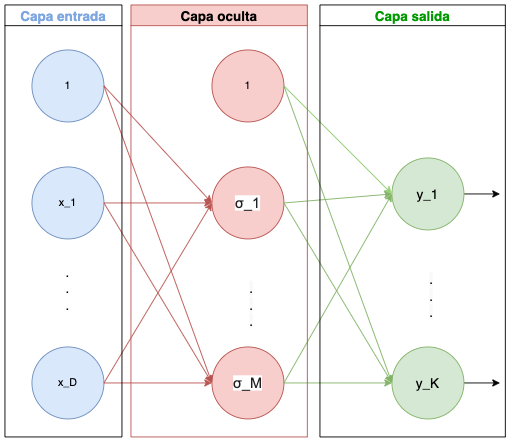
\includegraphics[width=0.65\textwidth]{introduccion_redes_neuronales/construccion_redes_neuronales/red-neuronal-simple-introduccion.drawio.png}
    \caption{Ejemplo de red neuronal con una capa oculta}
    \label{img:ejemplo topología red neuronal}
\end{figure} 
 

En este ejemplo poseemos una capa oculta, 
puede definirse siguiendo esta misma idea
una red neuronal de múltiples capas ocultas. 

% Generalización de modelo 
\subsection{Construcción red neuronal de varias capas ocultas} \label{rrnn:construcción_generalizada}

Etiquetaremos a cada capa con $l \in \{0, \ldots, L \}$, donde $L+1$ es el número total de capas.  Donde 

\begin{itemize}
    \item La capa de entrada será la etiquetada con $l = 0$.
    \item La capa de salida que determina el valor de la red neuronal es la $l=L$.
    \item Las capas ocultas serán aquellas etiquetadas como $0 < l <L.$
\end{itemize}

Se usará un superíndice para hacer referencia a la capa. 
Cada capa posee una dimensión $d^{(l)}$, es decir que posee
$d^{(l)} + 1$ unidades o nodos. El nodo $d_0^{(l)}$ se trata del sesgo y siempre será uno. 

El modelo de red neuronal $\mathcal{H}_{n n}$ viene determinado una vez que se fija la arquitectura de la misma, es decir sus dimensiones $d$. 
\begin{equation}
    d = (d^{(0)}, d^{(1)}, \ldots, d^{(L)})
\end{equation}
y se tiene que cada red neuronal $h \in \mathcal{H}_{n n}$
viene determinada por sus pesos. 

\subsubsection*{Cálculo de una capa oculta}  
Cada nodo recibe una señal de entrada $s$ y determina una salida $x$. 
  
La relación que existe entre dos nodos de capas contiguas es la siguiente: si $x_i^{(l-1)}$ es la salida de la unidad $i$ de la capa $l-1$, 
entonces se calcula la entrada de la unidad $j$ de la capa $l$ como 
\begin{align}\label{eq:construcción_red_neuronas:calculo_una_capa_oculta}
    s_j^{(l)} &= w_{i j}^{(l)} \cdot x_i^{(l-1)}  \\
    x_j^{(l)} &= \theta(s_j^{(l)})
\end{align}

Es decir, que en cada capa $l$ intervienen los siguientes elementos:  
\begin{table}[h]
    \begin{center}
    \begin{tabular}{| l | l | l |}
    \hline
    Elementos & Notación & Representación 
    \\ \hline
    Vector de entrada & $s^{(l)}$ &  Vector de dimensión $d^{(l)}$ \\
    Vector de salida & $x^{(l)}$ &  Vector de dimensión $d^{(l)}+ 1$ \\
    Pesos entrada & $W^{(l)}$ & Matriz de dimensiones $(d^{(l-1)}+1) \times d^{(l)}$ \\
    Pesos salida & $W^{(l+1)}$ 
    & Matriz de dimensiones $(d^{(l)}+1) \times d^{(l+1)}$ \\
    \hline
    \end{tabular}
    \caption{Elementos capa oculta $l$}
    \label{tab:rrnn_elementos_capa_oculta}
    \end{center}
\end{table}

\subsection{ \textit{Forward propagación}}

Explicaremos en esta sección cómo calcular para una entrada una determinada salida, es decir
dada una red neuronal $h \in \mathcal{H}_{d^{(0)} \times \cdots \times d^{(L)}}$ y un vector de entrada $x \in \mathcal{X}$ calcularemos  $h(x)$, esto se hará gracias al algoritmo conocido como \textit{forward propagation}.

Teniendo presente la relación  explicada en (\refeq{eq:construcción_red_neuronas:calculo_una_capa_oculta}) se puede escribir de forma vectorial la siguiente relación: 
\begin{equation}
    x^{(l)} = 
    \left[ \begin{array}{c}
        1 \\
       \theta(s^{(l)})
        \end{array}
\right] .
\end{equation}
Donde $\theta(s^{(l)})$ es un vector de componentes $\theta(s^{(l)}_j)$. 
Para calcular el vector de entrada de la capa $l$, para cada nodo se hará
\begin{equation}
    s_j^{(l)} = \sum_{i=0}^{d^{(l-1)}} w_{i j}^{(l)}x_i^{(l-1)}.
\end{equation}
Que se formula de forma vectorial para toda la capa como 
\begin{equation}
    s^{(l)} = W^{(l)} x^{(l-1)}.
\end{equation}

Si el vector de entrada es $x \in \mathcal{X} \subseteq \R^d$, 
se inicializa  $x^{(0)} = (1,x_1, \ldots, x_d)^T$ y por tanto $d^{(0)} = d+1.$


La implementación del algoritmo sería:

\begin{algorithm}[H]
    \caption{Algoritmo \textit{Forward propagation} para evaluación de una red neuronal $h_w(x)$.}
    \begin{algorithmic}[1]
        \STATE $x^{(0)} \leftarrow x$ 
        \COMMENT{Inicialización}

        \STATE \COMMENT{\textit{Forward Propagation}}
        \For{$l = 1, \ldots , L$}{
            % Calcula s
            \STATE 
            \begin{equation}
                s^{(l)}
                    \leftarrow
                    \left(W^{(l)}\right)^T
                    x^{(l-1)}      
            \end{equation}

            %Calcula x
            \STATE
            \begin{equation}
                x^{(l)}
                    \leftarrow
                    \left[ 
                        \begin{array}{c}
                            1 \\ 
                            \theta \left( s^{(l)}\right)
                        \end{array}
                    \right]
            \end{equation}
        }
        \STATE $h_w(x) = x^{(L)}$ 
        \COMMENT{Salida}  
\end{algorithmic}
\end{algorithm}

% Imagen red neuronal con pesos concretos
Veamos un ejemplo concreto para la siguiente red neuronal de la imagen \ref{img:construccion_rrnn:rrnn-2-3-2-1}
\begin{figure}[h!]
    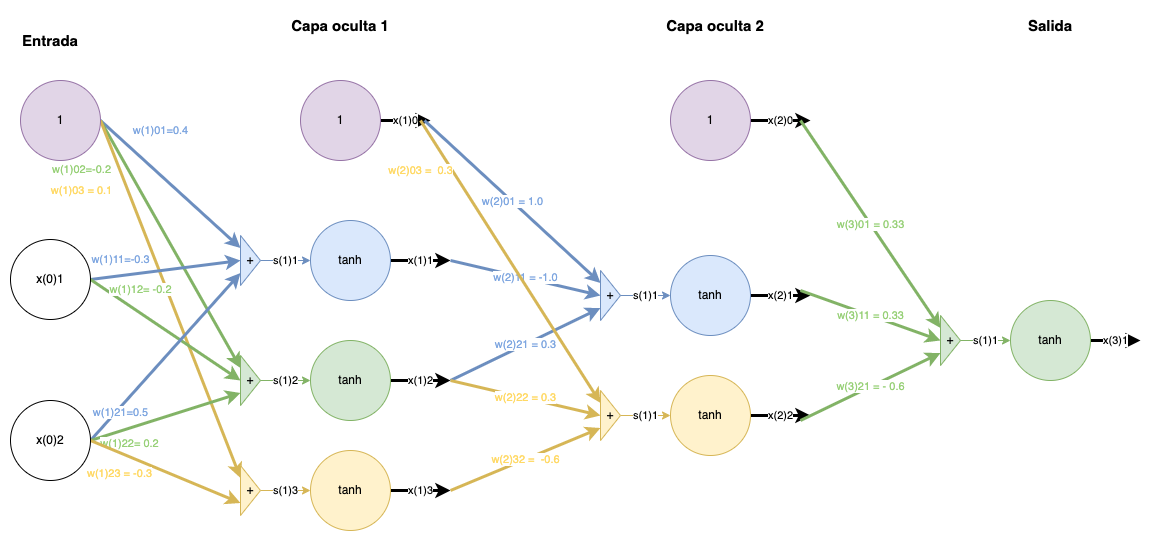
\includegraphics[width=\textwidth]{introduccion_redes_neuronales/construccion_redes_neuronales/rrnn-2-3-2-1-completa.png}
    \caption{Ejemplo de red neuronal con dos capas ocultas y pesos con valores concretos}
    \label{img:construccion_rrnn:rrnn-2-3-2-1}
\end{figure} 

La red de la imagen \ref{img:construccion_rrnn:rrnn-2-3-2-1} está 
compuesta por dos capas ocultas, acepta vectores de entrada de dimensión dos, 
la primera capa oculta está compuesta por tres neuronas, 
la segunda por dos y la salida por una. 
La notación del dibujo usada es la siguiente, entre paréntesis se 
especifica la capa, en el caso de la salida $x(l)i$ hace referencia a la salida $i$-ésima de la capa $l$. Las \textit{flechas} que conectan los nodos $w(l)ij$ hace referencia al peso que se le da a $x(l-1)i$ con respecto a la entrada $s(l)j$.

Representando los pesos de manera matricial
\begin{align}
    W^{(l)} = 
    \begin{bmatrix}
        w^{(l)}_{01} & w^{(l)}_{11} & \cdots & w^{(l)}_{d^{(l-1)} 1}\\
        w^{(l)}_{02} & w^{(l)}_{12} & \cdots & w^{(l)}_{d^{(l-1)} 2}\\
        \cdots & \cdots & \cdots & \cdots \\
        w^{(l)}_{0d} & w^{(l)}_{1d} & \cdots & w^{(l)}_{d^{(l-1)} d}\
    \end{bmatrix} 
\end{align}
las matrices de pesos de nuestra imagen son :
\begin{align}
    W^{(1)} = 
    \begin{bmatrix}
        0.4 & -0.3 & 0.5\\
        -0.2 & -0.2 & 0.2\\
        0.1 & 0 & -0.3
    \end{bmatrix} ,
    W^{(2)} = 
    \begin{bmatrix}
        1 & -1 & 0.3 & 0\\
        0.3& 0 & 0.3 & -0.6 
    \end{bmatrix} ,
    W^{(3)} = 
    \begin{bmatrix}
        0.33 & 0.33 & -0.6 \
    \end{bmatrix} .
\end{align}
Si inicializamos $x= (1,0)$ y tomamos como función de activación
a la tangente hiperbólica, la ejecución del algoritmo queda reflejada en la tabla \ref{tab:construcción_rnnn:ejemplo_forward_propagation} resultando que 
$h((1,0)) = 0.439$.
\begin{table}[H]
    \begin{center}
\begin{tabular}{| c | c | c | c| }
    \hline
    Capa $l$-ésima &  $W^{(l)}$ & $\bigl(s^{(l)}\bigr)^T $ & $\bigl(x^{(l)}\bigr)^T$ \\ \hline
    0 & & & $(1,1,0)$ 
    \\ \hline
    1 & 
    $\begin{bmatrix}
        0.4 & -0.3 & 0.5\\
        -0.2 & -0.2 & 0.2\\
        0.1 & 0 & -0.3
    \end{bmatrix}$ 
    & $(0.1, -0.4, 0.1)$ & $(1, 0.1, -0.38, 0.1)$
     \\ \hline
    2 & $\begin{bmatrix}
        1 & -1 & 0.3 & 0\\
        0.3& 0 & 0.3 & -0.6 
    \end{bmatrix}$
    & $(0.786, 0.126)$
    & $(1,0.656, 0.126)$
    \\ \hline
    3 & $\begin{bmatrix}
        0.33 & 0.33 & -0.6 
    \end{bmatrix}$ 
    & $(0.471)$ 
    & $(1,0.439)$
    \\ \hline
\end{tabular}
\caption{Ejemplo de ejecución del algoritmo de \textit{forward propagation}}
\label{tab:construcción_rnnn:ejemplo_forward_propagation}
\end{center}
\end{table}

%%%%%%%%%%%%%%%%%%% algoritmo de gradiente descendente 

\subsection{El gradiente descendente} \label{sec:gradiente-descendente}

(Información tomada de los capítulos uno y dos de \cite{learning-from-data-1-2})
Así pues, una vez concretado el problema y sus elementos 
(\ref{sub:componentes_aprendizaje}) es necesario definir un método con el que aproximar la función ideal $f,$ para ello introduciremos el algoritmo de gradiente descendente.  

El gradiente descendente es un método iterativo de minimización de funciones diferenciables. 

En nuestro caso particular se quiere aproximar la función ideal desconocida $f$ a partir de funciones (redes neuronales) $h_w \in \mathcal{H}$, donde $w \in M(\R)_{m \times n}$ son parámetros que caracterizan a $h_w$.
Para  
Dada también una función de error diferenciable y que no presente puntos de inflexión
$E: M(\R)_{m \times n} \longrightarrow \R,$
se toma una matriz inicial  cualquiera $w_0 \in M(\R)_{m \times n}$ y 
fijado $\eta \in \R^+$. 

Se define la sucesión 
\begin{equation}
    w_{t+1}  = w_t - \eta \nabla E(w_t).
\end{equation}  

Donde $w_n$ es una sucesión cuyos términos convergen a un mínimo local.
\subsubsection*{Observaciones sobre el algoritmo }

\begin{itemize}
    \item El algoritmo solo encuentra óptimos locales con una dependencia crucial del valor de inicio. 
    \item La convergencia no es segura en un tiempo finito y requiere de criterios de parada. 
    \item Si la función es convexa el mínimo será global.
    \item El parámetro $\eta$ puede ser cualquiera y debe de ser fijado o controlado por el diseñador.  
\end{itemize}




%%%%%%%%%% backpropagation 
\subsection{\textit{Backpropagation}}

Los parámetros que determinan una red neuronal son sus pesos, y esto es lo que \textit{aprende},
para actualizarlos utilizaremos la técnica de gradiente descendente ya explicado en la sección \ref{sec:gradiente-descendente}. 

\begin{equation}
    W(t+1) = w(t) - \eta \nabla E_{in}(w(t)). 
\end{equation}

Además, con el fin de reducir el coste del cálculo del gradiente, 
se utiliza el algoritmo conocido como \textit{backpropagation} que fue publicado en 
1989 en el artículo \cite{backpropagation-Hinton}. 

Sea $E_{in}(w)$ la función de error, la cual tomaremos como el error dentro de conjunto de entrenamiento, esto es,  si el conjunto 
de entrenamiento está constituido por $N$ datos de la forma $(x_n, y_n)$ con $x_n$ el vector de entrada y $y_n$ el estado o valor deseado para cualquier $n\in \{1, \ldots, N\}.$
\begin{equation}
    E_{in}(w) = \frac{1}{N} \sum^N_{n=1} (h_w(x)- y_n)^2. 
\end{equation}
Denotaremos como $e_n$ a 
\begin{equation}
    e_n = (h_w(x)- y_n)^2 
\end{equation}
que es una métrica para medir error entre, en nuestro caso  
la red neuronal $h_w$ y los valores deseados, con $w$ el vector que contiene las respectivas matrices de pesos de cada capa 
$W^{(l)} l \in \{1, \ldots, L\}.$  

%% Ejemplo 
Mostraremos un ejemplo primero antes de presentar el método general para facilitar la comprensión del algoritmo. 
% Imagen red neuronal simple
\begin{figure}[h!]
    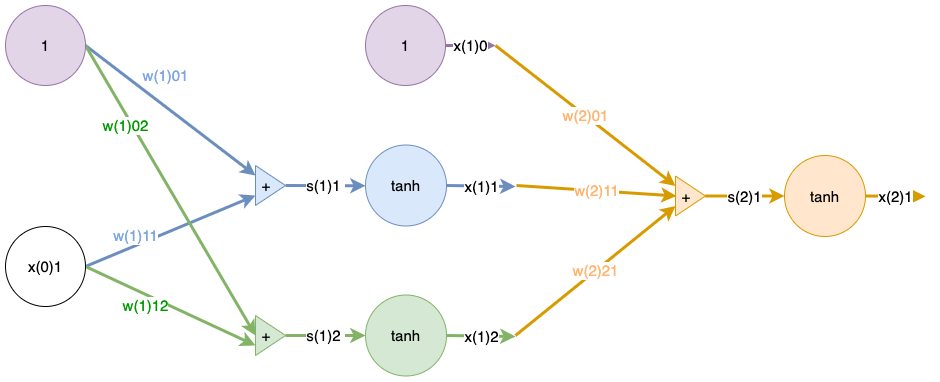
\includegraphics[width=\textwidth]{introduccion_redes_neuronales/construccion_redes_neuronales/rrnn-1-2-1.drawio.png}
    \caption{Red neuronal con una capa oculta a la que se quiere aplicar \text{backpropagation}}
    \label{img:construccion_rrnn:rrnn-1-2-1}
\end{figure} 
Queremos actualizar los pesos $w$ de la red neuronal 
$f_w : \R \longrightarrow \R$ presentada en \ref{img:construccion_rrnn:rrnn-1-2-1}.
$f_w$ está compuesta de dos capas ocultas. Supongamos que nos basaremos en un dato 
$(x, y)$ así pues podemos suponer que 
\begin{equation}
    E_{in}(w) = \frac{1}{N}e(f_w(x), y) = \frac{1}{N} (f_w(x)- y)^2.
\end{equation}
Como queremos actualizar los pesos utilizando el método de gradiente descendente necesitamos calcular el gradiente $\nabla E_{in}(w)$, en nuestro caso tenemos $w=\{W^{(1)}, W^{(2)}\}$ con 
\begin{align}
    W^{(1)} = 
    \begin{bmatrix}
        w^{(1)}_{01} & w^{(1)}_{11} \\
        w^{(1)}_{02} & w^{(1)}_{12} \\
    \end{bmatrix} 
    \text{ y }
    W^{(2)} = 
    \begin{bmatrix}
        w^{(2)}_{01} & w^{(2)}_{11} & w^{(2)}_{21}\\
    \end{bmatrix}, 
\end{align}
luego 
\begin{equation}
    \nabla E_{in}(w) = 
    \left(
        % primera capa 
        \frac{\partial e}{\partial w^{(1)}_{01}},
        \frac{\partial e}{\partial w^{(1)}_{11}},
        \frac{\partial e}{\partial w^{(1)}_{02}},
        \frac{\partial e}{\partial w^{(1)}_{12}},
        % segunda capa
        \frac{\partial e}{\partial w^{(2)}_{01}},
        \frac{\partial e}{\partial w^{(2)}_{11}},
        \frac{\partial e}{\partial w^{(2)}_{21}}
    \right).
\end{equation} 
Cada parcial se calcula, utilizando la regla de la cadena como
\begin{align}
    \frac{\partial e}{\partial w^{(1)}_{01}} 
    &=
    \frac{\partial e}{\partial s_1^{2}}
    \frac{\partial s_1^{2}}{\partial w^{(1)}_{01}} 
    \\
    &= 
    \frac{\partial }{\partial w^{(1)}_{01}}
         \tanh \left(s^{(2)}_{1}\right)
    \\
    &= 
    \left(1- \tanh^2 \left(s^{(2)}_{1}\right)\right) 
    \frac{\partial s^{(1)}_{1}}{\partial w^{(1)}_{01}}
    \\
    &= 
    \left(1- \tanh^2 \left(s^{(2)}_{1}\right)\right) 
    \frac{\partial }{\partial w^{(1)}_{01}}
    \left(w^{(2)}x^{(1)}\right)
    \\
    &= 
    \left(1- \tanh^2 \left(s^{(2)}_{1}\right)\right) 
    \frac{\partial }{\partial w^{(1)}_{01}}
    \left(
        \sum^2_{i=0}
        w^{(2)}_{i1}x^{(1)}_i
    \right)
    \\
    &= 
    \left(1- \tanh^2 \left(s^{(2)}_{1}\right)\right) 
    \left(
        \sum^2_{i=0}
        w^{(2)}_{i1}\frac{\partial x^{(1)}_i }{\partial w^{(1)}_{01}}
    \right)
    \\
    &= 
    \left(1- \tanh^2 \left(s^{(2)}_{1}\right)\right) 
    \left(
        \sum^2_{i=1}
        w^{(2)}_{i1}\frac{\partial }{\partial w^{(1)}_{01}}
        \left(
            \tanh \left(s^{(1)}_{i}\right)
        \right)
    \right)
    \\
    &= 
    \left(1- \tanh^2 \left(s^{(2)}_{1}\right)\right) 
    \left(
        \sum^2_{i=1}
        w^{(2)}_{i1}
        \left(
            \left(1- \tanh^2 \left(s^{(1)}_{i}\right)\right)
            \frac{\partial  }{\partial w^{(1)}_{01}}
            \left(
                \sum^1_{j=0}\sum^2_{k=1}
                w^{(1)}_{j k}x^{(0)}_j
            \right)
        \right)
    \right)
    \\
    &= 
    \left(1- \tanh^2 \left(s^{(2)}_{1}\right)\right) 
    \left(
        \sum^2_{i=1}
        w^{(2)}_{i1}
        \left(
            \left(1- \tanh^2 \left(s^{(1)}_{i}\right)\right)
            x^{(0)}_0
        \right)
    \right).
\end{align}
Notemos que no se han evaluado las apariciones de $s_i^{(j)}$.
Otro ejemplo sería
\begin{align}
    \frac{\partial e}{\partial w^{(2)}_{21}} 
    &=
    \frac{\partial }{\partial w^{(2)}_{21}}
         \tanh \left(s^{(2)}_{1}\right)
    \\
    &= 
    \frac{\partial }{\partial w^{(2)}_{21}}
         \tanh \left(w^{(2)}x^{(1)}\right)
    \\
    &= \left(
    1- \tanh^2 \left(s^{(2)}_{1}\right) \right)x^{(1)}_2.
\end{align}

Notemos que no se han desarrolla los términos de la forma $s^{(i)}_j$. Además si existen $Q$ pesos la complejidad del cálculo será $\mathcal{O}(Q^2)$, sin embargo, como hemos visto existen términos que se repiten en ambas ecuaciones, por lo que utilizar una técnica de programación dinámica, concretamente la conocida como 
\textit{backpropagation} (\cite{backpropagation-Hinton}) nos permite reducir el coste a una complejidad de  $\mathcal{O}(Q).$

%% Fin del ejemplo 
%% COMIENZA EL ARTÍCULO 

%Formalizaremos primero qué parámetros debemos estimar del gradiente.

Sea $\theta$ una función de activación derivable, 
 $L$ el número de capas ocultas, $N$ el tamaño del conjunto de entrenamiento $x^{(0)} = (1, x_1, \ldots, x_{d^{(0)}})^T$ 
siendo $x = (x_1, \ldots, x_{d^{(0)}})^T$ la entrada de la red neuronal, $x^{(L)}$ la salida de la red neuronal y 
$d^{(l)}$ la dimensión, número de nodos en la capa $l$-ésima. 
Recordemos que 
para cualquier $l \in \{1, \ldots, L\}$ con
\begin{equation}
    x^{(l)}
     = 
     \theta \left( s^{(l)}\right) 
     = 
     \theta \left( W^{(l)} x^{(l-1)}\right),
\end{equation}
y
\begin{equation}
    E(w) = \frac{1}{N} 
    \sum_{n = 1}^{N}
    \sum_{i = 1}^{d^{(L)}}
    \left({x_n}^{(L)}_i-y_{n_i} \right)^2 
    = 
    \frac{1}{N}
    \sum^{N}_{n=1} e_n.
\end{equation}

%% Gradiente de la salida: 
Para simplificar la notación nos referiremos como $e$ a $e_n.$
Vamos a proceder a calcular primero los gradientes de la última capa, 
sea $w^{(L)}_{i j}$  con $j \in \{1, \ldots , d^{(L)}\}$, 
$i \in \{1, \ldots , d^{(L-1)}\}$  el peso que relaciona la salida 
$x_i ^{(L-1)}$ del  
nodo $i$ de la capa anterior con la entrada $s_j ^{(L)}$ del nodo $j$ de la última capa. 
Vamos a calcular $\frac{\partial e}{ w^{(L)}_{i j}}$ utilizando la regla de la cadena. 
\begin{equation}
    \frac{\partial{e}}{\partial w^{(L)}_{i j}}
     = 
     \frac{\partial{e}}{\partial x^{(L)}_j} 
     \frac{\partial x^{(L)}_j}{\partial s^{(L)}_j} 
     \frac{\partial s^{(L)}_j}{\partial w^{(L)}_{i j}}.
\end{equation}
Donde es fácil ver que para el tercer término
\begin{equation}\label{eq:backpropagation_s_última_capa_derivada}
    \frac{\partial s^{(L)}_{j}}{\partial w^{(L)}_{i j}}
    = 
    \frac{\partial }{\partial w^{(L)}_{i j}}
    \left(
        w^{(L)}_{\ast j } \cdot x^{(L-1)}
    \right)
    = 
    x^{(L-1)}_j
\end{equation}
Donde $w^{(L)}_{\ast j} = \left(w^{(L)}_{0 j}, w^{(L)}_{2 j}, \ldots, w^{(L)}_{d^{(L-1)} j}\right)$ representa los pesos correspondientes al nodo $j$,
 en forma de  vector fila y $x^{(L-1)} = \left(1, x ^{(L-1)}_1, \ldots, x ^{(L-1)}_{d^{(l-1)}}\right)^T$ el valor de la salida de la capa $L-1$
 en forma de vector columna.
 
 Por otro lado 
 \begin{equation}\label{eq:backpropagation_E_última_capa_derivada}
    \frac{\partial{e}}{\partial x^{(L)}_j} =
    2 
    \left(
    x^{(L)}_j - y_j
    \right)
 \end{equation}
 donde conocemos $x^{(L)}_j$ gracias al algoritmo de \textit{forward propagation}
 y $y_j$ la componente $j$-ésima del vector deseado en el entrenamiento.
y finalmente
\begin{equation}\label{eq:backpropagation_x_última_capa_derivada}
    \frac{\partial x^{(L)}_j}{\partial s^{(L)}_j} 
    = 
    \frac{d}{d s^{(L)}_j} 
        \theta \left( 
            s^{(L)}_j
        \right)
\end{equation}
que sabemos que se puede calcular por ser $\theta$ derivable y 
$s^{(L)}_j$ un valor conocido que ya ha sido calculado por el algoritmo de 
\textit{forward propagation.}

Por lo tanto, concluimos por 
(\refeq{eq:backpropagation_E_última_capa_derivada}),
(\refeq{eq:backpropagation_x_última_capa_derivada})
y  
(\refeq{eq:backpropagation_s_última_capa_derivada})
\begin{equation}
    \frac{\partial{e}}{\partial w^{(L)}_{i j}}
     = 
     \frac{\partial{e}}{\partial x^{(L)}_j} 
     \frac{\partial x^{(L)}_j}{\partial s^{(L)}_j} 
     \frac{\partial s^{(L)}_j}{\partial w^{(L)}_{i j}} 
    =
    2\left( x^{(L)}_j - y_j \right) 
    \theta' \left( s^{(L)}_j\right)
    x^{(L)}_j.
\end{equation}
%%%% Gradiente interior 
Denotaremos por \textit{sensibilidad} a 
\begin{equation}
    \delta^{(l)} = \frac{\partial e}{ \partial s^{(l)}}.
\end{equation}

Para calcular la derivada de pesos de capas interiores 
$l \in \{1 \ldots L-1\}$
procederemos de la siguiente manera, para 
$j \in \{1, \ldots , d^{(l)}\}$ y 
$i \in \{1, \ldots , d^{(l-1)}\}$ 
\begin{equation}
    \frac{\partial{e}}{\partial w^{(l)}_{i j}}
     = 
     \frac{\partial e}{\partial s^{(l)}_j} 
     \frac{\partial s^{(l)}_j}{\partial w^{(l)}_{i j}}
    = 
    \delta^{(l)}
    \frac{\partial}{\partial w^{(l)}_{i j}}
    w^{(l) \cdot x^{(l-1)}}
    = 
    \delta^{(l)} x^{(l-1)}_i,
\end{equation}
donde  $x^{(l-1)}_i$ es conocida por el algoritmo de 
$\textit{forward propagation}$. 

Por otra parte 
$\delta^{(l)}_j$ 
cumple que 
\begin{align}
    \delta^{(l)}_j 
    &= 
    \frac{\partial e}{\partial s^{(l)}_j}
    \\
    &= 
        \frac{\partial e}{\partial s^{(l+1)}}
        \frac{\partial s^{(l+1)}}{\partial s^{(l)}_j}
    \\
    &= 
    \delta^{(l+1)} 
    \frac{\partial}{\partial s^{(l)}_j}
        \left( w^{(l)} \cdot \theta(s^{(l)})\right)
    \\
    &= 
    \delta^{(l+1)}_j 
    w^{(l)}_j \cdot  \theta'(s^{(l)}_j). 
\end{align}
Por lo que de forma matricial tenemos que $\delta^{(l)}$ 
cumple que 
\begin{align}
    \delta^{(l)} 
    &= 
    \frac{\partial e}{\partial s^{(l)}}
    \\
    &= 
        \frac{\partial e}{\partial s^{(l+1)}}
        \frac{\partial s^{(l+1)}}{\partial s^{(l)}}
    \\
    &= 
    \delta^{(l+1)} 
    \otimes 
    \frac{\partial}{\partial s^{(l)}}
        \left( w^{(l)} \cdot \theta(s^{(l)})\right)
    \\
    &= 
    \delta^{(l+1)} 
    \otimes 
    \left(
    w^{(l)} \cdot \theta'(s^{(l)})
    \right). 
\end{align}

De esta manera a partir de las \textit{sensibilidades} de las 
capas posteriores es posible calcular las $l$-ésimas y puesto que 
la sensibilidad $\delta_{(L)}$ es conocida acabamos de determinar 
cómo calcular la derivada de todos los pesos  de manera constructiva. 
Procedemos a explicitar los cálculos. 

\subsubsection{Algoritmos para la actualización de los pesos}  

El razonamiento expuesto conduce al siguiente proceso algorítmico 
para el cálculo de los gradientes. 

% pseudo código cálculo de sensibilidades 
\begin{algorithm}[H]
    \caption{Algoritmo \textit{backpropagation} para calcular
    las sensibilidades $\delta^{(l)}$}
    \hspace*{\algorithmicindent} \textbf{Input}: un par de $(x,y)$ del conjunto de entrenamiento.  \\
    \hspace*{\algorithmicindent} \textbf{Output} 
    \begin{algorithmic}[1]
        % Forward propagation
        \STATE Se ejecuta el algoritmo de \textit{forward propagation} 
        
        con $x$ como entrada para calcular y guardar : 
        \begin{align}
            s^{(l)} \quad &\text{for } l = 1, \ldots, L;
            \\
            x^{(l)} \quad &\text{for } 0 = 1, \ldots, L;
        \end{align}
        % Inicializamos
        \STATE \COMMENT{Inicializamos sensibilidades últimas capas}
        \begin{equation}
            \delta^{(L)} \longleftarrow 2
            \left( 
                x^{(L)} - y
            \right)
            \theta' \left( s^{(L)} \right)
        \end{equation}
        \STATE 
        \COMMENT{ \textit{Backpropagation}}
        
        \For{$l = L-1$ to $1$}
        {
            \begin{equation}
                \delta^{(l)} 
                    \leftarrow
                \theta' 
                \left(
                    s^{(l)}
                \right)
                \otimes
                \left[
                    W^{(l+1)}
                    \delta^{(l+1)}
                \right]^{d^{(l)}}_1
            \end{equation}
        }
\end{algorithmic}
\end{algorithm}

% pseudo código cálculo cálculo de gradiente  
\begin{algorithm}[H]
    \caption{Algoritmo para el cálculo $E_{in}(w)$
    y $g = \nabla E_{in}(w).$}
    \hspace*{\algorithmicindent} \textbf{Input}:
    $w = \left\{ W^{(1)}, \ldots, W^{(L)}\right\};$
    $\mathcal{D} = (x_1, y_1), \ldots, (x_n, y_n).$\\
    \hspace*{\algorithmicindent} \textbf{Output:} error $E_{in}(w)$ y gradiente
    $g = \{G^{(1)}, \ldots, L\}.$  
    \begin{algorithmic}[1]
        \STATE Inicializamos $E_{in}(w)=0$ y $G^{(l)} = 0$ 
        for $l = 1, \ldots, L.$
        \STATE \For{ cada punto $(x_n, y_n),$
        n = 1, \ldots, N}{
            % cálculos de las x^l y sensibilidades
            \STATE Calcula $x^{(l)} \quad \text{for } l = 1, \ldots, L;$
            \COMMENT{ \textit{forward propagation}}
            \STATE Calcula $\delta^{(l)} \quad \text{for } l = L, \ldots, 1;$
            \COMMENT{ \textit{backpropagation}}
            % vamos sumando el erro en cada punto 
            \STATE
            \begin{equation}
                E_{in} 
                \leftarrow
                E_{in} + 
                \frac{1}{N}(x^{L}-y_n)^2 
            \end{equation}
            \For{l=1, \ldots, L}{
                \STATE
                \COMMENT{Calculamos gradiente en un punto}
                \begin{equation}
                    G^{(l)}\left( x_n\right) = 
                    \left[
                        x^{(l-1)}
                        \left(
                            \delta^{(l)}
                        \right)^T
                    \right]
                \end{equation}
                \STATE 
                \begin{equation}
                    G^{(l)}
                    \leftarrow
                    G^{(l)}
                    + 
                    \frac{1}{N}
                    G^{(l)}\left( x_n\right)
                \end{equation}
            }
        }
\end{algorithmic}
\end{algorithm}

Finalmente para conocer el valor actualizado de los pesos, lo actualizaremos usando la técnica de gradiente descendente. 

\begin{algorithm}[H]
    \caption{Algoritmo gradiente descendente.}
    \hspace*{\algorithmicindent} \textbf{Input}: Pesos $w$ y gradiente $g$. \\
    \hspace*{\algorithmicindent} \textbf{Output:} $w$ actualizado
    \begin{algorithmic}[1]
        \STATE
        \For{$l = 1, \ldots, L.$}{
            \begin{equation}
                W^{(l)}
                \leftarrow
                W^{(l)} 
                - 
                \eta G^{(l)}                    
            \end{equation}
        }
\end{algorithmic}
\end{algorithm}
